\documentclass[11pt, a4paper]{article}

% --- PACCHETTI ---
\usepackage[margin=2.5cm]{geometry} 
\usepackage{graphicx} 
\usepackage{hyperref} 
\usepackage{float} 

\title{Relazione Progetto CCAI}
\author{Vincenzo Rubulotta, Paola Pappalardo, Lorenzo Varsallona}
\date{} 

\begin{document}

\maketitle

\section{Introduzione e Scenario}

Il presente documento descrive la progettazione, l'implementazione e la valutazione di un sistema di Intelligenza Artificiale basato su agenti, sviluppato per il corso CCAI. Il progetto mira a realizzare un sistema agentico calato nello scenario di supporto per un blogger. 

Per soddisfare questo requisito, abbiamo scelto di focalizzarci sul dominio gastronomico, implementando un sistema multi-agente di supporto per un blog di cucina intelligente. L'obiettivo dell'agente è generare autonomamente ricette e contenuti culinari sempre nuovi, garantendo un'alta qualità editoriale ed evitando la ripetizione di argomenti o piatti già proposti di recente tramite l'utilizzo di un dataset vettoriale e un knowledge graph popolato dinamicamente.

L'architettura del sistema integra organicamente le tre competenze fondamentali richieste: il ragionamento agentico, l'utilizzo di una componente semantica K-RAG (Knowledge Graph-augmented RAG) e il fine-tuning di un modello linguistico di grandi dimensioni (LLM). La base di conoscenza combina in modo sinergico un Knowledge Graph editoriale per la gestione dei dati strutturati e un database vettoriale per il recupero di contenuti non strutturati, permettendo al sistema di espandere le query e validare le informazioni estratte.

\subsection{Tecnologie Utilizzate}

Lo sviluppo dell'intero ecosistema ha richiesto l'integrazione di diversi framework, database e modelli, selezionati per garantire modularità, scalabilità e prestazioni elevate:

\begin{itemize}
    \item \textbf{LangGraph}: Framework di orchestrazione principale utilizzato per definire e gestire il flusso di lavoro multi-agente attraverso un'architettura a grafo direzionato, regolata da nodi e archi condizionali.
    \item \textbf{Neo4j}: Database a grafi nativo impiegato per ospitare la struttura semantica del Knowledge Graph editoriale, consentendo la memorizzazione e l'interrogazione delle relazioni e delle triple estratte dalle ricette.
    \item \textbf{ChromaDB}: Database vettoriale open-source utilizzato come memoria locale per l'indicizzazione dei documenti e per abilitare le funzionalità di recupero semantico dense della componente RAG.
    \item \textbf{Cohere}: Suite di modelli integrata nella pipeline di recupero per eseguire operazioni di Reranking avanzato, ottimizzando la pertinenza dei contesti estratti prima di sottoporli alla generazione.
    \item \textbf{Groq e Llama 3.1:70b}: Piattaforma di inferenza ad altissima velocità utilizzata per servire il modello open-weight Llama 3.1 da 70 miliardi di parametri, impiegato come motore di ragionamento logico primario dell'architettura.
    \item \textbf{Dataset ISMEA}: Base di dati istituzionale integrata nel sistema per estrarre informazioni strutturate sui prezzi di mercato dei prodotti agroalimentari, tracciare dinamiche economiche e suggerire alternative biologiche.
    \item \textbf{Dataset Custom (Giallozafferano)}: Base di conoscenza documentale creata ad hoc per il progetto tramite attività di web scraping sul portale gastronomico Giallozafferano, contenente un ampio ricettario testuale esteso utilizzato per alimentare il database vettoriale.
\end{itemize}

\subsection{Struttura del Grafo Multi-Agente}

Il flusso di lavoro dell'agente, dalla pianificazione editoriale alla fase di stesura e revisione dei post (Human-in-the-loop), è stato modellato attraverso una serie di nodi e archi condizionali. In questo processo, l'agente mantiene in memoria lo stato interno a ogni step (ragionamento, pianificazione e output) e giustifica le proprie scelte in modo dinamico.

La Figura \ref{fig:graph} illustra l'architettura a nodi del sistema implementato.

\begin{figure}[H] 
    \centering
    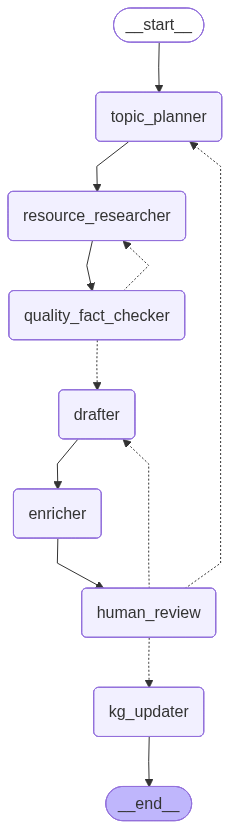
\includegraphics[width=0.2\textwidth]{images/graph.png}
    \caption{Architettura a nodi del sistema multi-agente per il blog di cucina.}
    \label{fig:graph}
\end{figure}

\section{Tool a Supporto dell'Agente}

Per portare a termine le proprie attività, l'architettura sfrutta il ragionamento dinamico (es. ReAct) per selezionare ed eseguire un set di strumenti in base al task corrente. 

Oltre ai tool fondamentali per l'esplorazione, il recupero e l'aggiornamento della base di conoscenza, l'ecosistema del nostro agente è stato arricchito con moduli personalizzati e verticalizzati sul dominio culinario ed editoriale. Di seguito viene presentata una panoramica sintetica degli strumenti a disposizione del sistema:

\begin{itemize}
    \item \textbf{\texttt{kg\_rag\_tool}}: Gestisce il recupero avanzato del contesto combinando dati strutturati e testi estesi attraverso una pipeline di Hybrid Search (Dense + BM25), fusione RRF e Cohere Reranking.
    \item \textbf{\texttt{aggiorna\_knowledge\_graph\_db}}: Assicura l'aggiornamento incrementale della base di conoscenza ibrida K-RAG. Salva i documenti vettorializzati nel database vettoriale e sfrutta un LLM per estrarre dinamicamente relazioni fondamentali (triple), fonti e topic, popolando strutturalmente il Knowledge Graph.
    \item \textbf{\texttt{cerca\_nel\_database\_ismea}}: Strumento custom focalizzato sulla dimensione economica e gastronomica della ricetta; interroga i dati sui prezzi e sulle alternative biologiche, suggerendo i vini ideali grazie a un LLM interno addetto al ragionamento e alla gestione dei dialetti locali.
    \item \textbf{\texttt{valuta\_documento\_locale} (Fact Checker Tool)}: Un modulo di controllo critico incaricato di analizzare semanticamente i testi delle ricette estratte localmente, validandone la reale pertinenza rispetto al \textit{target topic} richiesto.
    \item \textbf{\texttt{cerca\_e\_leggi\_sul\_web} (Web Tool)}: Consente l'estrazione e lo scraping multi-pagina dal web per raccogliere informazioni esterne aggiornate, garantendo un controllo incrociato e la verifica dell'accuratezza delle fonti.
\end{itemize}

Il funzionamento dettagliato, le interazioni e le logiche interne di ciascun tool verranno approfonditi nei prossimi paragrafi.

\end{document}